\documentclass[mathserif,usenames,dvipsnames]{beamer}
\usepackage{algorithmic}
%\usetheme{Bergen}
%\usetheme{Copenhagen}
% \usetheme{Darmstadt}
% \usetheme{Frankfurt}
%\usetheme{Luebeck}
\usetheme{Madrid}
\usecolortheme{beetle}
%\usefonttheme{serif}
%\usecolortheme{dove}
%\usecolortheme{fly}
%\usecolortheme{seagull}
%\useinnertheme{rectangles}
%\useinnertheme{circles}
%\useinnertheme{inmargin}
%\useinnertheme{rounded}
%% =======================================================
%% (c) Tobias Schoofs
%% =======================================================
%% Commands 4 Programmers
%% =======================================================

%include lhs2TeX.fmt
%include lhs2TeX.sty

%\usepackage[pdftex]{graphicx}
%\usepackage{ucs}
%\usepackage[utf8x]{inputenc} 
\usepackage{tabto}
\usepackage[russian,portuguese,german,english]{babel}
\usepackage{CJK}
\usepackage{amsfonts}
\usepackage{amsfonts}

\usepackage{amsmath}
\usepackage{amssymb}
\usepackage{amsthm}
\usepackage{amscd}

\usepackage{siunitx}

\usepackage{listings}
\usepackage{longtable}

\usepackage{tikz}
\usepackage{pgfplots}

\usepackage{relsize}
\usepackage{xcolor}

\usepackage{soul}

\long\def\ignore#1{}

\newcommand{\acronym}[1]{\textsc{#1}}

\newcommand{\term}[1]{\textit{#1}}
\newcommand{\tech}[1]{{\ttfamily #1}}
\newcommand{\latin}[1]{\textit{#1}}
\newcommand{\speech}[1]{\textit{#1}}

\newcommand{\ie}{\textit{i.e.}}
\newcommand{\eg}{\textit{e.g.}}
\newcommand{\etc}{\textit{etc.}}
\newcommand{\viz}{\textit{viz.}}
\newcommand{\vs}{\textit{vs.}}

\newcommand{\sql}{\acronym{sql}}

\newcommand{\code}[1]{{\ttfamily #1}}
\newcommand{\cmdline}[1]{{\ttfamily #1}}

\newenvironment{sqlcode}{
\small
\begin{minipage}{\textwidth}
\lstset{language=sql,
        keepspaces=true,
        showspaces=false,
        showstringspaces=false}
}{
\end{minipage}
}

\newenvironment{python}{
\small
\begin{minipage}{\textwidth}
\lstset{language=python,
        keepspaces=true,
        showspaces=false,
        showstringspaces=false}
}{
\end{minipage}
}

\newenvironment{ccode}{
\small
\begin{minipage}{\textwidth}
\lstset{language=C,
        keepspaces=true,
        showspaces=false,
        showstringspaces=false}
}{
\end{minipage}
}

\newcommand{\keyword}[1]{\textbf{#1}}
\newcommand{\identifier}[1]{\textit{#1}}

\newcommand{\Rom}[1]{\uppercase\expandafter{\romannumeral #1\relax}}

\newcommand{\CC}{C\nolinebreak[4]\hspace{-.05em}\raisebox{.3ex}{\relsize{-2}{\textbf{++}}}}
\newcommand\csharp{C\nolinebreak[4]\hspace{-.02em}\raisebox{.3ex}{\relsize{-1}{\#}}}

\newcommand{\comment}[1]{\textcolor{red}{#1}}

\newcommand{\nowdb}{\textsc{n}o\textsc{wdb}}

\newcommand{\connect}[2]{
  \draw [-,color=black] (#1) to (#2)
}

% tikz
% \newcommand{\drawDataPoint}{\draw circle (0.2)}
% \drawDataGroup

% \renewcommand{\gcd}{\textsc{gcd}}

\title{What is \nowdb?}
\author{Tobias Schoofs}
\begin{document}

% TITLE
\frame{\titlepage}

% OVERVIEW 
\begin{frame}
\frametitle{Overview}
\begin{itemize}
\item What?
\item Why?
\item How?
\item Vision!
\item Market!
\item Where are we now?
\item What means the name?
\end{itemize}
\end{frame}

% WHAT
\begin{frame}
\frametitle{What?}
\begin{equation*}
\nowdb = (graph +  timeseries + \acronym{sql}) \times (Python + Lua)
\end{equation*}
\end{frame}

% WHY TIMESERIES
\begin{frame}[shrink]
\frametitle{Why Timeseries?}
\begin{itemize}
\item Growing amount of data that are timeseries \emph{to some extent}
\item Important driver: \acronym{i}o\acronym{t}
\item But also: ``traditional'' industries:
      \begin{itemize} 
      \item \acronym{it} infrastructure providers,
      \item Energy,
      \item Manufacturing (``Industry 4.0'')
      \item Retail
      \item \dots
      \end{itemize}
\item Timeseries data have special requirements:
      \begin{itemize}
      \item Fast ingestion ($> 1M/s$)
      \item Scalability of queries ($> 1B metrics$)
      \item Special handling of time dimension
      \item Timeseries are less rigid compared to relational data\\
            (time points may be lost or duplicated)
      \end{itemize}
\item Avalailable timeseries databases
     (\eg\ \acronym{i}nflux\acronym{db}, \acronym{o}pen\acronym{tsdb}) are too narrow, 
      \ie\ \emph{pure} timeseries.
\item There are projects trying to solve this issue,
      \eg: \[
      timescale = postgres + timeseries\]
      $\dots$ but it's still Postgres: somewhat slow
\end{itemize}
\end{frame}

% WHY GRAPH
\begin{frame}
\frametitle{Why Graph?}
\begin{columns}[T]
\column{0.75\linewidth}
\begin{itemize}
\item Make timeseries more widely applicable!
\item Natural candidates: Relational and Graph
\item Graph is more flexible:\\
      we can add new edges \\
      without changing the structure of entities
\item Graph is less rigid:\\
      edges pointing to nowhere or\\
            pointing to duplicated data are no issue
\item Graph may be easier to grasp:\\
      and this way reduce common errors in data modelling.\\
      (This, however, is pure speculation on my side $\dots$)
\end{itemize}
\column{0.25\linewidth}
\vskip1cm
\hskip-0.2\linewidth
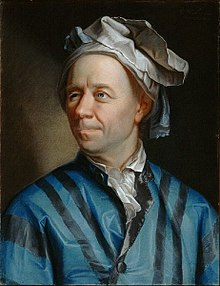
\includegraphics[width=0.75\linewidth]{leoeuler.jpg}
\end{columns}
\end{frame}

% WHY SQL
\begin{frame}
\frametitle{Why \acronym{sql}?}
\begin{itemize}
\item \st{Make }\acronym{\st{sql}}\st{ great again!}
\item \acronym{sql} is standard.
\item \acronym{sql} is actively developed with new ideas flowing in.
\item \acronym{sql} is known by virtually everybody in the industry.
\item \acronym{sql} is easy to learn (even though tricky to master \dots)
\item \acronym{sql} is designed for integration with other languages and tools.
\item \acronym{sql} is supported by thousands of tools.
\item \acronym{sql} is not bad anyway.
\item Well \dots
\item Next slide!
\end{itemize}
\end{frame}

% Why Python?
\begin{frame}[shrink]
\frametitle{Why Python?}

\includegraphics[width=0.2\linewidth]{pythonlogo.png}
\begin{itemize}
\item An important application domain is data science.
\item There will be demand for tools, libraries, languages supporting
\begin{itemize}
\item Statistics
\item Calculus
\item Numerical analysis
\item Function analysis and function plotting
\item Linear algebra (vectors, matrices, \etc)
\item Graph(!)-oriented data structures
\item \dots
\end{itemize}
\item Millions of lines of code available in (or through) Python
\item Python is \textbf{the} data science language.\\
      (There also is $R$, but $R$ is very limited as general purpose language)
\item It is in particular interesting to have Python available
      on server side.
      This will reduce client/server round trips
      and network traffic.
\end{itemize}
\end{frame}

% Why Lua?
\begin{frame}[shrink]
\frametitle{Why Lua?}
\begin{columns}[T]
\column{0.9\linewidth}
\begin{itemize}
\item Python has an issue with its interpreter:
      \begin{itemize}
      \item difficult to run many interpreters ($=$ sessions)
      \item in parallel in one process ($=$ \nowdb\ server).
      \end{itemize}
\item In consequence:
      Python is not good for tasks that frequently run
      in parallel.
\item We therefore need a second language for more
      down-to-earth, day-to-day \acronym{dba} jobs.
\item Lua appears to be a good candidate because:
\begin{itemize}
\item Lua is well known in the data science community
\item Lua already had its appearance on the database stage\\
      (namely in the redis \term{in-memory} database)
\item Lua is designed as configuration language\\
      (and \acronym{dba} tasks are often configuration tasks)
\item Lua is designed for integration with the C language.
\end{itemize}
\end{itemize}
\column{0.18\linewidth}
%\begin{flushright}
\vskip5cm
\hskip-0.5\linewidth

\includegraphics[width=0.8\linewidth]{lualogo.png}
%\end{flushright}
\end{columns}
\end{frame}

% HOW
\ignore{
datamodel example with
simple edges:
- product of category or
- client has address
timeseries edges:
- client buys product
on joins
select client.buys.destin
}
\begin{frame}
\frametitle{How? Data Modelling}
\begin{columns}[T]
\column{0.33\linewidth}
\begin{center}
\vskip0.5cm
The Relational Way\\
\vskip1cm
\hspace*{1.2cm}
%\includegraphics[width=1.2\linewidth]{relational.png}
\begin{tikzpicture}
\draw (0,3) rectangle (1,1.5);
\draw (0,3) rectangle (1,2.6);
\node [font=\tiny,align=center] (sup) at (0.5,2.8) {Supplier};
\node [font=\tiny,align=center,anchor=west] (sup1) at (0,2.3) {\textbf{id}};
\node [font=\tiny,align=center,anchor=west] (sup2) at (0,2.0) {name};
\node [font=\tiny,align=center,anchor=west] (sup3) at (0,1.7) {\dots};

\draw (3,2) rectangle (4,0);
\draw (3,2) rectangle (4,1.5);
\node [font=\tiny,align=center] (prod) at (3.5,1.75) {Product};
\node [font=\tiny,align=center,anchor=west] (sup1) at (3,1.2) {\textbf{id}};
\node [font=\tiny,align=center,anchor=west] (sup2) at (3,0.9) {desc};
\node [font=\tiny,align=center,anchor=west,text=red] (sup2) at (3,0.6) {supplier};
\node [font=\tiny,align=center,anchor=west] (sup3) at (3,0.3) {\dots};

\draw (1,2.3) -- (1.75,2.3) -- (1.75,0.6) -- (3,0.6);
\node [font=\tiny,align=center,anchor=west] (one) at (1,2.4) {1};
\node [font=\tiny,align=center,anchor=west] (n) at (2.6,0.7) {$n$};
\end{tikzpicture}
\end{center}
\column{0.33\linewidth}
\begin{center}
The Logical Fact\\[12pt]
%\includegraphics[width=0.9\linewidth]{logic.png}
\begin{tikzpicture}
\draw (0.1,2.3) circle (0.1cm); % head
\draw (0.1,2.2) -- (0.1,1.8);   % body
\draw (-0.1,2.1) -- (0.3,2.1);  % arms
\draw (0.1,1.8) -- (-0.1,1.5);  % left leg
\draw (0.1,1.8) -- (0.3,1.5);   % right leg
\node [font=\tiny,align=center] (sup) at (0.1,1.3) {Supplier};

\draw (1.9,2.3) circle (0.1cm); % head
\draw (1.9,2.2) -- (1.9,1.8);   % body
\draw (1.7,2.1) -- (2.1,2.1);   % arms
\draw (1.9,1.8) -- (1.7,1.5);  % left leg
\draw (1.9,1.8) -- (2.1,1.5);   % right leg
\node [font=\tiny,align=center] (prod) at (1.9,1.3) {Product};

\draw [->] (0.5,1.9) -- (1.5,1.9);  % edge
\node [font=\tiny,align=center] (edg) at (1.0,1.7) {supplies};
\end{tikzpicture}
\end{center}
\column{0.33\linewidth}
\begin{center}
\vskip0.5cm
The Graph Way\\
\vskip1cm
%\hskip-0.5\linewidth
\hskip-2.7cm
%\includegraphics[width=1.2\linewidth]{graph.png}
\begin{tikzpicture}
\draw (3,3) rectangle (4,1.5);
\draw (3,3) rectangle (4,2.6);
\node [font=\tiny,align=center] (sup) at (3.5,2.8) {Supplier};
\node [font=\tiny,align=center,anchor=west] (sup1) at (3,2.3) {\textbf{id}};
\node [font=\tiny,align=center,anchor=west] (sup2) at (3,2.0) {name};
\node [font=\tiny,align=center,anchor=west] (sup3) at (3,1.7) {\dots};

\draw (0,2) rectangle (1,0);
\draw (0,2) rectangle (1,1.5);
\node [font=\tiny,align=center] (prod) at (0.5,1.75) {Product};
\node [font=\tiny,align=center,anchor=west] (sup1) at (0,1.2) {\textbf{id}};
\node [font=\tiny,align=center,anchor=west] (sup2) at (0,0.9) {desc};
\node [font=\tiny,align=center,anchor=west] (sup3) at (0,0.6) {\dots};

\draw [->] (3,2.3) -- (2,2.3) -- (2,1.2) -- (1,1.2);
\node [font=\tiny,align=center,anchor=west] (origin) at (2.05,2.4) {$origin$};
\node [font=\tiny,align=center,anchor=west] (destin) at (0.98,1.32) {$destin$};
\end{tikzpicture}
\end{center}
\end{columns}
\end{frame}

% SQL Example
\begin{frame}[fragile]
\frametitle{How? Graph}
\begin{columns}[T]
\column{0.4\linewidth}
\vskip0.5cm
{\small Create a vertex type}
\vskip1.7cm
{\small Create another vertex type}
\vskip1.7cm
{\small Add an edge \\without changing the types}
\column{0.5\linewidth}
\begin{sqlcode}
\begin{lstlisting}
create type supplier (
  id uint primary key,
  name text,
  ...
);
create type product (
  id uint primary key,
  description text,
  ...
);
create edge supplies (
  origin supplier,
  destin product
);
\end{lstlisting}
\end{sqlcode}
\end{columns}
\end{frame}

% Timeseries
\begin{frame}[fragile]
\frametitle{How? Timeseries}
\begin{columns}[T]
\column{0.4\linewidth}
\vskip0.5cm
{\small Product type}
\vskip1.7cm
{\small Client type}
\vskip1.7cm
{\small Timeseries edge}
\column{0.5\linewidth}
\begin{sqlcode}
\begin{lstlisting}
create type product (
  id uint primary key,
  description text,
  ...
);
create type client (
  id uint primary key,
  name text,
  ...
);
create edge buys (
  origin client,
  destin product,
  timestamp time,
  quantity float,
  price    float
);
\end{lstlisting}
\end{sqlcode}
\end{columns}
\end{frame}

% Query
\begin{frame}[fragile]
\frametitle{How? Queries (1/2)}
\begin{columns}[T]
\column{0.25\linewidth}
\vskip0.5cm
{\small Who bought product 12345?}\\
{\tiny  (This query runs in ms!)}
\vskip1.0cm
{\small Traditional Join}
\vskip1.9cm
{\small Implicit join}
\column{0.75\linewidth}
\begin{sqlcode}
\begin{lstlisting}
select origin
  from buys
 where destin = 12345
   and year(stamp) = 2018
   and month(stamp) >= 10;

select p.description
  from buys (join product as p on destin)
            (join client  as c on origin)
 where c.name = 'Smith'
   and year(stamp) = 2018;

select destin.description
  from buys
 where origin.name = 'Smith'
   and year(stamp) = 2018;
\end{lstlisting}
\end{sqlcode}
\end{columns}
\end{frame}

% Query 2
\begin{frame}[fragile]
\frametitle{How? Queries (2/2)}
\begin{columns}[T]
\column{0.25\linewidth}
\vskip0.3cm
{\small Who are the suppliers of products bought by client 'Smith'?}
\vskip0.7cm
{\small Can we use \acronym{cte} for recursive search on paths?}\\
{\small Well \dots}\\
{\small Next Slide!}
\column{0.75\linewidth}
\begin{sqlcode}
\begin{lstlisting}
select destin.supplies.origin.name
  from buys
 where origin.name = 'Smith'
   and year(stamp) = 2018;

with path (n,e) as (
  select 1, origin.friend
    from friend
   where origin.name = 'Smith' 
     and year(stamp) = 2018
  union
  select n+1, destin.friend
    from friend
   where year(stamp) = 2018
     and n < 10)
select count(*)
  from path
 where origin.name = 'Muller';
\end{lstlisting}
\end{sqlcode}
\end{columns}
\end{frame}

% Storage engine
\begin{frame}
\frametitle{How? Storage Engine (1/2)}
Two storage types:
\begin{enumerate}
\item Edge Store:
      \begin{itemize}
      \item optimised for fast ingestion
      \item data packed to favour typical queries
      \item special handling of timestamps
      \item small memory footprint
      \item optional compression
            (recommended for timeseries edges)
      \end{itemize}
\item Vertex Store:
      \begin{itemize}
      \item consistent data (no duplicates)
      \item column-oriented
            (\ie\ optimised for large data types)
      \item enforce primary key
      \item in-memory caches to speed up
            inserts and queries
      \item optional compression
            (recommended only for large tables)
      \end{itemize}
\end{enumerate}
\end{frame}

\begin{frame}
\frametitle{How? Storage Engine (2/2)}
Four index types:
\begin{enumerate}
\item Primary Keys (Vertex)
      \begin{itemize}
      \item B$^+$Tree
      \item storing set of \term{pageids}
      \end{itemize}
\item Secondary Vertex Index
      \begin{itemize}
      \item B$^+$Tree
      \item storing set of primary keys
      \end{itemize}
\item Page Index (Edge):
      \begin{itemize}
      \item B$^+$Tree
      \item storing ``embedded'' B$^+$Trees
            storing pageids
      \item used for queries and joins on edges
      \end{itemize}
\item Label Index (Edge):
      \begin{itemize}
      \item B$^+$Tree
      \item storing fixed number of pageids
      \item used to find related edges
      \end{itemize}
\end{enumerate}
\end{frame}

% VISION
\begin{frame}[shrink]
\frametitle{Vision!}
\begin{itemize}
\item \textbf{Scalability!}\\
      Reduce hardware and software license cost
      by allowing more data to be stored on one node,
      \ie\ billions of metrics per server.
\item \textbf{Data Analysis}\\
      Provide server- and client-side Python modules
      to ease data science.
\item \textbf{Integration with big-data tools}\\
      Ease big-data by integration with existing tools
      \eg\ Kafka for reliable ingestion of data.
\item \textbf{Integration with distribution engines}\\
      Ease large-scale computation by integration with existing tools
      \eg\ \acronym{spark} for distributed computing.
\item \textbf{Integration with visualisation frameworks}\\
      Ease application development by integration with existing
      \acronym{gui} frameworks, \eg\ Grafana.
\item \textbf{Integration with traditional tools}\\
      Use \acronym{odbc/jdbc} to make the platform available
      to traditional tools.
\item \textbf{Publish/Subscribe Capability}\\
      Provide pub/sub capability to ease the development
      of monitoring and real-time data analysis.
\end{itemize}
\end{frame}

% MARKET
\begin{frame}
\frametitle{Market!}
\begin{itemize}
\item \textbf{Complement} existing \acronym{oltp} infrastructures
\item \textbf{Compete} with complex big-data and data science platforms
      providing a low-cost alternative 
      to frameworks with high cost of ownership
      (\eg: Hadoop, large \acronym{olap} systems, \etc)
\item Target industries with ``timeserish'' data 
      and need of data science
      (\eg\ \acronym{i}o\acronym{t}, retail, fintech, ``Industry 4.0'')
\item Provide pre-packaged out-of-the-box solutions
      (\eg\ integration with Kafka, Zookeeper, \acronym{spark} \& Grafana)
\item Operate with a mix of open-source and proprietary licenses
      (\eg\ generic modules for free, specific modules for pay)
\item Foster a community among customers to grow repository of
      available solutions and modules
\item Foster community of \term{certified} service providers
\end{itemize}
\end{frame}

% WHERE ARE WE NOW 
\begin{frame}[shrink]
\frametitle{Where are we now? (1/2)}
\begin{itemize}
\item Prototype is available:
      \bgroup
      \setbeamercolor{item}{fg=green}
      \begin{itemize}
      \item Client/Server
      \item \acronym{sql} with many operators and functions:
            \begin{itemize}
            \item arithmetic and boolean operators and functions,
            \item \acronym{case} and other conditionals,
            \item time and geospatial functions,
            \item trigonometry,
            \item string operators and functions,
            \item \dots
            \end{itemize}
      \item Python client- and server-side
      \item Simple command line client
      \setbeamercolor{item}{fg=yellow}
      \item First iteration of Grafana plug-in
      \item Foundations for grouping, ordering and joins
      \item Storage engine needs revision
      \item User manual on the way
      \setbeamercolor{item}{fg=red}
      \item Query planner still rudimentary
      \item Todo: security and user management
      \end{itemize}
      \egroup
\end{itemize}
\end{frame}

\begin{frame}[shrink]
\frametitle{Where are we now? (2/2)}
\begin{columns}[T]
\column{0.75\linewidth}
\begin{itemize}
\item We are currently working with the \acronym{i}o\acronym{t}
      startup \textbf{Loka Systems} (\url{https://loka.systems})
      to identify strengths and weaknesses.
      \begin{itemize}
      \item The Loka database has about 30M metrics
      \item It was imported into \nowdb\ in $< 30s$
      \item Queries were implemented by means of\\
            server-side Python modules
      \item Results are visualised by Grafana and Plotly
      \item The feedback of the Loka team already led
            to conceptional and technical improvements
      \end{itemize}
\item We created a database with data
      by the World Meteorological Organisation
      (\acronym{wmo})
      \begin{itemize}
      \item with weather data covering the years 1970 -- 2018
      \item with more than 1B metrics
      \item Import takes about 5 minutes
      \item Index-based queries run in milliseconds
      \item Benchmarks reveal some weaknesses \\
            (\eg\ grouping)
      \end{itemize}
\end{itemize}
\column{0.25\linewidth}
\begin{center}
\hskip-0.5\linewidth

\includegraphics[width=0.85\linewidth]{lokalogo.png}
\vskip0.85cm
\hskip-0.4\linewidth

\includegraphics[width=0.85\linewidth]{grafanalogo.png}
\vskip1.0cm
\hskip-0.4\linewidth
{\color{MidnightBlue} \url{www.wmo.int}}
\end{center}
\end{columns}
\end{frame}

% NORBERT WIENER
\begin{frame}
\frametitle{The funny Name}
\begin{columns}[T]
\column{0.4\linewidth}
\begin{itemize}
\item a reference to time
\item a pun on \term{no}\acronym{sql} and \term{new}\acronym{sql}
\item \dots and a homage to Norbert Wiener,\\
      the father of \\ timeseries analysis \\
      for Control \& Communication
\end{itemize}
\column{0.6\linewidth}
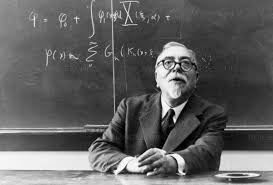
\includegraphics[width=\linewidth]{wiener.jpeg}
\end{columns}
\end{frame}
\end{document}
